%!TEX program = xelatex
% 完整编译: xelatex -> bibtex -> xelatex -> xelatex
\documentclass[lang=cn,11pt,a4paper]{paper}

\title{地方补贴式租赁住房的挤出效应:来自LIHTC计划的新证据}
\author{Michael D. Eriksen\thanks{\href{http://www.eriksen.myweb.uga.edu}{迈克尔·D·埃里克森},电话:+1 706 542 9774,传真:+1 706 542 4295,电子邮件:\email{eriksen@terry.uga.edu}。佐治亚大学特里商学院房地产系,美国乔治亚州雅典城,GA 30602。} \and Stuart S. Rosenthal\thanks{\href{http://www.faculty.maxwell.syr.edu/rosenthal}{斯图亚特·S·罗森塔尔},通讯作者,电话:+1 315 443 3809,传真:+1 315 443 1081,电子邮件:\email{ssrosent@maxwell.syr.edu}。锡拉丘兹大学经济系和政策研究中心,美国纽约锡拉丘兹,13244-1020。}\; \thanks{\href{https://www.sciencedirect.com/science/article/pii/S0047272710000885}{\faIcon{link} 英文原文链接}。作者非常感谢约翰·D·凯瑟琳·麦克阿瑟基金会,福特基金会以及住房和城市发展部为该项目提供的资金。本文从许多个人的有益评论中受益。我们感谢两位匿名编辑Dennis Epple(编辑),Denise DiPasquale,Gary Engelhardt,Jeffrey Kubik,Edgar Olsen,Erika Poethig,Steve Ross,Michael Stegman,Bruce Weinberg,Johnny Yinger,以及参加2007年1月AREUEA会议和俄亥俄州立大学提供有用的意见。当然,文责自负。}}
\translator{翻译者:\href{https://tomben.me/}{任\ 涛}}

%\version{0.08}
\date{\zhtoday}

\begin{document}

\maketitle

\begin{abstract}
  \hspace{2\ccwd}自1987年成立以来,低收入住房税收抵免(LIHTC)计划已迅速发展成为美国有史以来最大的低收入住房补贴建筑来源,占最近所有多户出租建筑的三分之一。本文研究了这种日益重要的中低收入住房来源的挤出效应。为此,我们分析了LIHTC建设对地理的三个不同层次(MSA,县和10英里半径圆)的影响。这使我们能够采用越来越广泛的地域固定效应,以帮助区别未观察到的因素。政治变量也被用作进一步促进识别的工具。
  
  \!在我们所有的模型中,IV估计产生的拥挤要比OLS大得多,这证实了LIHTC开发对新建筑成熟区域的内生吸引力。我们最可靠的IV估算表明,LIHTC发展的近100\%被 新建的无补贴租赁单位的数量,尽管这一点估计值附近的置信区间允许进行不太剧烈的评估。其他估算表明,LIHTC的发展对自住房建设的影响要小得多,但这些估算并不精确。总体而言,尽管LIHTC的发展可能会很好地影响低收入公寓的位置,但我们的估计表明,该计划对新开发的出租房屋数量的影响似乎很小。

  \keywords{挤出效应,保障性住房,LIHTC}
\end{abstract}
\vspace{10pt}

\begin{tcolorbox}[
	colback=yellow!10!white,
  colframe=red!30!black,
  fontupper = \itshape,
]
“I rise today to introduce the Affordable Housing Tax Credit Enhancement Act of 2005. … the bill would double the current LIHTC [annual allocations], which would yield twice the number of affordable units annually. … Today, the LIHTC program is widely regarded as the nation's most successful housing production program resulting in the construction and rehabilitation of more than 1.3 million housing units for lower income households. …”
\vspace{5pt}

\textbf{Statements Submitted to Congressional Record: May 26, 2005 By Rep. William Jefferson (D-LA)}

\tcblower

“我今天起草来介绍《2005年经济适用房税收抵免增强法案》。……该法案将使目前的LIHTC(年度拨款)翻一番,这将使每年的经济适用房数量增加一倍。 …今天,LIHTC计划被公认为是美国最成功的住房生产计划,它为低收入家庭建造和修复了130万套住房……”
\vspace{5pt}

\textbf{众议员William Jefferson(D-LA)在2005年5月26日提交国会记录的声明。}

\end{tcolorbox}
\vspace{10pt}

\section{引言}

提供给穷人的住房援助的方式仍然有很多甚至是激烈的争论:政府应该通过需求方优惠券类型计划(例如第8节优惠券)还是通过公共和低价等供应方建筑补贴在地方投资人 收入住房税收抵免(LIHTC)住房? 在此背景下,本文考察了快速增长的LIHTC计划,并强调了LIHTC建设在多大程度上排除了无偿租赁房屋的开发。 一些进一步的背景将有助于使LIHTC计划成为现实。

在1930年代末至1980年代中期,联邦政府通过“传统”公共住房计划建造了超过一百万套住房。 重要的是,这些计划通常将入住人数限制在贫困线以下或以下的家庭 \citep{Olsen2003365}\,\footnote{\cite{Olsen2003365}指出,至少有29种不同的公共住房计划。 这些项目中的家庭通常将其总收入的30\%用于租金。}。到1980年代,至少在两个方面,人们的担忧开始削弱对公共住房进一步扩大的支持。 首先是政府建设,拥有和运营公共住房项目。 关于某些活动是否最好留给私营部门存在一些基本问题。 第二个是公共住房项目造成了密集的贫困集群,加剧了人们对犯罪,邻里衰落以及对项目中儿童成长的不利影响的担忧,例如可参见 \cite{Currie200099,Jencks1990111}。出于这些原因,公共住房的建设在1980年代初结束了,1990年代开始拆除性能最差的项目\,\footnote{在某些情况下,例如根据HOPE VI计划,公共住房结构进行了改建,但在大多数情况下,通常向住户发放住房券,并告知他们私下寻求住房 \cite{Jacob2004233}。}。

随着1986年的税收改革法案(TRA86),低收入住房税收抵免(LIHTC)计划应运而生,作为公共住房的替代方案,同时也抵消了改革对出租住房业主的其他税收优惠的取消\citep{USCongress1987}\,\footnote{根据美国税法第42条,LIHTC计划由国内税收署管理。}。LIHTC项目的前提与公共住房明显不同,它是基于政府和营利性开发商之间的合作关系。根据LIHTC的规定,私人市场开发商可以从非土地建设成本中获得高额补贴,补贴的慷慨程度还会随着LIHTC为收入低于住房和城市发展部(HUD)规定标准的租户保留的公寓份额的增加而增加\,\footnote{联邦政府通过一项为期10年的年度不可退还的联邦所得税抵免,一美元一美元地降低私人开发商的联邦所得税责任,补贴私人开发商30 - 91\%的非土地建设成本 \cite{Eriksen2009141}。由于补贴的慷慨程度随着分配给低收入居民的项目单元份额的增加而增加,大多数开发商的应对措施是让所有单元都住满符合收入标准的租户。不遵守LIHTC的操作规则将导致开发商丧失未来的税收抵免,并偿还1/10。}。此外,开发商同意在至少15年内,将目标公寓的租金设定在规定的上限以下,之后才允许收取市场租金。考虑到这些规定,LIHTC在某些方面是一种有针对性的租金控制形式,其中资格规则限制占用。

LIHTC很快就超越了之前所有基于场所的补贴租赁项目,成为美国历史上最大的此类项目。在\tabref{tab1}中,值得注意的是,从1987年到2006年,大约建造了160万套LIHTC住房,占最近建造的多户出租住房的大约三分之一。\figref{fig1}进一步说明了这一点。这个数字显示了过去60年公共住房的建设和LIHTC的发展\,\footnote{用于创建\figref{fig1}的公共住房数据是从住房和城市发展部的分析师那里获得的,并得到了约翰·麦克阿瑟和凯瑟琳·麦克阿瑟以及阿布特协会的帮助。这些数据在两个方面不同于 \url{http://www.huduser.org} 的公开数据。首先,我们的数据包含每个“项目”从1937年到2000年投入使用的年份。这使我们能够代表每十年新建的公共住房。此外,我们的数据还包括1990年代拆除公共住房的信息。LIHTC数据是从 \url{http://www.lihtc.huduser.org} 的平显获得的。}。最近LIHTC发展的繁荣是显而易见的。同样显而易见的是,在\tabref{tab2}中,请注意,尽管LIHTC计划的成本相对于住房券计划来说似乎不算高,但LIHTC计划的绝对成本却很高。2006年,住房代金券项目耗资近210亿美元。相比之下,与LIHTC计划相关的联邦税收损失总计49亿美元。然而,由于从2001年开始分配的信贷增加了40\%,预计这一费用在未来几年将急剧增加\,\footnote{即使最近有关扩大LIHTC项目的提议尚未出台,这些增长也会发生。有关各种形式的低收入者住房支助费用的详细资料载于住房和城乡建设局的一份报告 \cite{USCongress2005}。}。


\begin{table}[h]
\centering
\setlength{\tabcolsep}{12mm}
  \begin{threeparttable}
  \caption{国家LIHTC汇总统计\tnote{a}}\label{tab1}
    \begin{tabular}{ccc}
  \toprule
  & 年度拨款总额 (\$)\tnote{b}
  & 补贴单位数量\tnote{c} \\
  \midrule
  1987 & 980,533,493 & 34,491 \\
  1988 & 3,140,987,971 & 81,408 \\
  1989 & 4,387,952,511 & 126,200 \\
  1990 & 2,888,647,156 & 74,029 \\
  1991 & 5,207,469,242 & 111,970 \\
  1992 & 4,255,013,370 & 91,300 \\
  1993 & 5,205,992,598 & 103,756 \\
  1994 & 5,915,192,114 & 117,099 \\
  1995 & 4,892,206,044 & 86,343 \\
  1996 & 4,277,723,133 & 77,003 \\
  1997 & 4,225,625,522 & 70,453 \\
  1998 & 3,999,808,231 & 67,822 \\
  1999 & 3,983,473,499 & 62,240 \\
  2000 & 3,895,882,268 & 59,601 \\
  2001 & 4,624,992,306 & 67,261 \\
  2002 & 5,162,994,677 & 69,310 \\
  2003 & 5,507,541,467 & 73,877 \\
  2004 & 5,680,347,051 & 75,600 \\
  2005 & 5,556,042,690 & 70,630 \\
  2006 & 6,668,538,964 & 74,278 \\
  总计 & 90,456,964,308 & 1,594,671 \\
  \bottomrule
    \end{tabular}
  \begin{tablenotes}
    \footnotesize
    \item[a] 数据由国家住房当局全国委员会汇编。
    \item[b] 计算时假设通货膨胀率为3\%,并且在分配后的10年内将申请已分配的税收抵免。
    \item[c] 不包括未补贴的市场价格单位,有时包括在LIHTC补贴的房产中。
  \end{tablenotes}
\end{threeparttable}
\end{table}

\begin{figure}[h]
	\centering
	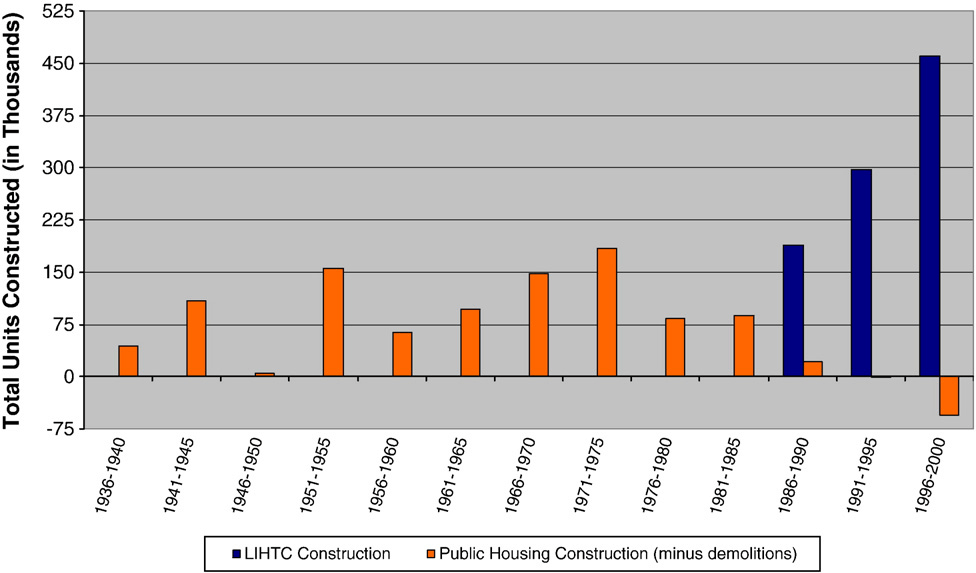
\includegraphics[width=13cm]{fig1.png}
	\caption{基于地点的住房补贴建造和拆除}\label{fig1}
\end{figure}


\begin{table}[h]
  \centering
  \setlength{\tabcolsep}{12mm}
    \begin{threeparttable}
    \caption{联邦政府低收入住房支出(2005-2006)(单位:百万美元)\!\!\tnote{a}}\label{tab2}
      \begin{tabular}{ccc}
        \toprule
        & 2005 & 2006 \\
        \midrule
        \textbf{国税局}\tnote{b} & & \\
        低收入住房税收抵免 & 4700 & 4900 \\
        优惠折旧免税额 & 3800 & 4200 \\
        国家发行的租赁住房免税融资 & 300 &
        300 \\[5pt]
        \textbf{住房和城市发展部}\tnote{c} & & \\
        住房选择券(HCV) & 20,064 & 20,917 \\
        公共住房 & 5017 & 5734 \\
        其他HUD项目 & 8734 & 4559 \\[5pt]
        \textbf{农业部}\tnote{c} & & \\
        农村住房管理 & 1369 & 1029 \\
        总计 & 43,984 & 41,639 \\
        \bottomrule
      \end{tabular}
    \begin{tablenotes}
      \footnotesize
      \item[a] LIHTC成本反映了与10年税收抵免分配相关的税收损失。鉴于自2001年以来LIHTC拨款的增加,这些费用预计将在未来几年大幅增加。随着越来越多的公共住房单元被拆除,未来几年公共住房运营成本可能会下降。
      \item[b] 根据 \cite{USCongress2005} 估算的税收支出。
      \item[c] 美国政府预算,\cite{Budget2006}。
    \end{tablenotes}
  \end{threeparttable}
  \end{table}


很明显,LIHTC是一个昂贵的项目。同样明显的是,LIHTC是一种有针对性的租金控制形式。不太明显的是,LIHTC的目标实际上是温和的,而不是低收入的租户。在考虑LIHTC计划的挤出效应时,这一点尤其重要,无论是在总体上还是在公共住房方面。尽管私营部门很少为接近或低于贫困线的家庭建造无补贴住房,但它经常建造中等收入的出租住房。这表明,虽然建造公共住房只是间接地与未受资助的私人开发项目竞争,但LIHTC项目与未受资助的建筑项目直接竞争。因为排挤是在政府与私营部门争夺市场份额时出现的,所以以中等收入家庭为目标增加了LIHTC项目取代无补贴开发的可能性。鉴于LIHTC计划的这一特点的重要性,我们在下面提供了四条证据,证实LIHTC倾向于以收入远高于传统公共住房的家庭为目标。

首先要考虑的一点是,LIHTC补贴住房的租金上限定得相对较高。准确地说,租金上限设定为家庭收入中位数,即生活津贴中位数)的18\%,每年由住房和城市发展部规定\,\footnote{之所以提出18\%的AMI收入门槛,是因为补贴单元的居住者的收入必须低于AMI的60\%,而向补贴单元的个人收取的租金不得超过该上限的30\%。}。尽管租金上限因城市而异,但它们与住房和城市发展部规定的公平市场租金想尽相近 \citep{Cummings1999257},后者用于管理第8节凭证领取者支付的租金。这些租金通常在上年私人市场合同租金的40\%至50\%之间。对于许多低收入家庭来说,这种水平的租金是负担不起的。

第二点也是相关的一点是,LIHTC补贴住房租户的收入限制也定在相对较高的水平。具体而言,住房和城市发展部将LIHTC补贴单位的收入资格定为最低收入水平的60\%。这一限额远远高于传统公共住房开发居住者的收入限额\,\footnote{例如,在2000年的华盛顿州DC市生活津贴中,住房和城市发展部为一个三口之家规定的LIHTC收入限额为43,500加元(大约相当于该规模家庭家庭收入中位数的60\%)。LIHTC项目业主在那一年可以向这样一个家庭收取的最高租金是每月1088美元。相比之下,2000年华盛顿州DC市的所有出租单元(未补贴加补贴单元)的租金中位数为每月840美元。参见住房和城市发展部网站:\url{http://www.huduser.org}。}。

第三点是关于LIHTC单位的建筑质量。针对高收入租户应该促使开发商提供更高质量的单元(因为住房是一种正常的商品)。\cite{Eriksen2009141} 使用1999年至2005年期间加州LIHTC发展的详细数据报告了与该结果一致的证据\,\footnote{\cite{Eriksen2009141} 还强调,由于LIHTC补贴非土地建设成本,而不是土地本身,要素价格替代效应应进一步鼓励开发商提高建设质量。}。\cite{Eriksen2009141} 发现LIHTC项目的非土地建设成本中位数为每平方英尺128美元。\cite{Eriksen2009141} 进一步报告说,这比加州同期无补贴租赁住房开发的非土地成本中位数高出21\%。

很明显,LIHTC的开发项目受到相对较高的租金上限、支配资格的高收入限制以及高质量的建筑的制约。综上所述,这些特征表明,LIHTC租户的收入可能比公共住房租户的收入要高得多。\cite{Wallace1995785} 发现,只有28\%的LIHTC居民的收入低于50\%的AMI (HUD用来定义非常低收入的家庭的基准),他认为,传统公共住房开发项目中81\%的居民收入非常低。鉴于上述证据和方案特点,很明显,LIHTC的目标是中等收入家庭,而不是低收入家庭。因此,LIHTC也有可能与未受资助的开发项目直接竞争,这增加了LIHTC项目取代未受资助建设项目的可能性。

为了评估LIHTC发展的挤出效应,我们将1990年的普查区域数据与1990年至2000年间LIHTC发展的信息相结合。我们的基本策略是对20世纪90年代LIHTC发展中的私营部门住房建设进行跨部门回归,控制先前文献中阐述的住房开工的其他驱动因素(例如 \cite{Mayer200085})。\cite{Murray1999107} 在分析美国住房总量的时间序列时强调的另一种方法是评估补贴住房建设对住房总量的影响。我们在论文的后面部分认为,我们对新发展的关注产生了密切相关的结果,这些结果在我们的数据具有很大的跨部门性质的情况下更加可靠。特别是,我们所有的模型都是以住房存量的滞后水平为条件的(以及其他将要描述的控制变量)。这使得我们的因变量反映了1990年至2000年期间住房存量的变化,而不管因变量是被指定为住房存量的变化还是2000年住房存量的水平\,\footnote{注意,以$y_t=b_0+b_1y_{t-1}+b_2x_t$为例,等式两边同时减去$y_{t-1}$,只影响滞后因变量的系数$x$不变。此外,\cite{Murray1999107} 试图分析保障性住房建设对住房均衡存量的影响,\cite{Murray1983590} 则侧重于保障性住房开发对住房开工率的影响。}。两个相关的经验挑战仍然存在,它们在我们识别挤出效应的努力中起着突出的作用。首先是选择分析LIHTC挤出效应的地理层次。第二是控制LIHTC发展可能是内生的可能性。我们在下面依次简要地考虑了每个问题,在本文后面会有进一步的细节。

出于几个原因,对LIHTC挤出效应的估计可能对分析LIHTC发展的地理水平敏感(例如,城市街区、县、MSA、州等)。首先,从概念的角度来看,被中低收入住房的潜在居民视为紧密替代品的社区属于一个共同的住房市场。因此,LIHTC在一个街区的开发将会降低共同市场中所有街区的均衡房价。当补贴活动压低了市场价格,迫使未补贴单元的开发商放弃供应职能时,挤出就发生了(详情将在本文后面提供)。这表明,对LIHTC挤出效应的全面核算要求地理分析单位足够大,以考虑到替代效应和相关的邻里价格效应。

然而,从经验的角度来看,增加分析单元的地理范围会减少可用于研究的位置的数量(例如,州比县少)。这导致数据的变化减少,使得识别挤出效应变得困难。在接下来的实证研究中,我们试图通过分别为三个不同的地理分析单元估计我们的模型来平衡这些抵消因素:MSA加上特定的农村地区、县和围绕2000年人口普查区域的地理中心画出的10英里半径的圆。这些地理层次中的每一个都给我们留下了深刻的印象,足以允许跨社区的实质性互动。每种方法的样本量和变异也不同,并且每种方法都提供了不同的机会来控制特定位置的因素。例如,我们在MSA级别的模型中包含州固定效果,但在10英里圆圈模型中使用县固定效果。后者要严格得多,在控制未观察到的因素方面走得更远,否则这些因素可能会使我们对挤出的估计产生偏差。

控制未补贴住房开发的未观察到的驱动因素的需要与我们对LIHTC发展的衡量是否是内生的这个问题密切相关,这是我们第二个主要的经验问题。一方面,开发商认识到资本收益的潜力因地点而异,这影响了LIHTC项目的预期回报。此外,如前所述,如果LIHTC投资者未能将项目单元的最低要求份额出租给收入低于住房和城市发展部规定限额的家庭,他们将受到严厉的经济处罚(埃里克森,2009年)。招致此类处罚的风险对租赁住房需求的波动很敏感,并且可能因地点而异。由于这些原因和其他原因,开发商可能会寻求将LIHTC项目定位在被认为是未来增长和新住宅建设时机成熟的地区。这将导致对LIHTC发展对私人非补贴建筑影响的普通最小二乘估计偏向更积极的价值,低估了LIHTC项目的挤出效应。另一方面,也有可能州政府官员在州政府分配的LIHTC信贷中进行监督,迫使开发商将项目建在压力很大的社区,否则很难在这些社区进行开发。这可能导致OLS的偏见走向相反的方向。综上所述,这些考虑表明,未能控制LIHTC项目的可能内生位置可能会使LIHTC挤出效应的估计产生偏差,尽管偏差的方向是不确定的,\textbf{是先验的}。

为了控制LIHTC单位的内生布局,我们在两阶段最小二乘程序中使用由管理LIHTC信贷分配的政治过程驱动的工具来为LIHTC发展提供工具。联邦法律指示国税局根据各州在美国人口中所占的比例在各州之间分配LIHTC信用额度,全国范围内的信用额度总数由国会设定。按照给定的州人口比例,我们假设1990年代对每个州的信贷总分配也是外生的。然后,在给定的年份里,各州使用各自认为合适的任何程序在各州内部重新分配学分(根据联邦整体计划的指导方针)。这些程序在不同的州和不同的时间有所不同,我们没有单个州/年分配程序的直接数据。相反,我们假设各州至少部分通过模仿联邦政府的政治过程来分配他们的信贷。具体而言,我们假设1990年至2000年间州内的信贷分配部分基于1990年某个特定地区(如县)的州人口份额。将1990年的当地人口份额乘以LIHTC信贷的国家分配,得出我们在给定地点的LIHTC单位数量的第一个工具。

作为第二个工具,我们考虑到任人唯亲也可能影响国家对宝贵的LIHTC补贴的分配。因此,对于每个县,我们基于该县是否在1989年投票给现任州长,编码一个等于1的虚拟变量。将这一衡量标准乘以上述第一个工具,就有可能使倾向于投票支持获胜州长候选人的社区获得的州LIHTC信贷份额高于其在州人口中所占份额的平均值\,\footnote{本文稍后将提供关于这些仪器的更多详细信息。就目前而言,这足以表明这些工具与LIHTC的发展密切相关(例如,\citep{Stock200580,Murray2006111}),并且过度识别限制的测试支持这两种工具的有效性,尽管我们对这种测试持谨慎态度,因为它们具有已知的弱功率以及假阴性和假阳性的趋势。}。

我们的主要结果表明,在县一级和10英里半径范围内,LIHTC开发产生的挤出效应接近100\%,尽管这些估计的标准误差足够大,可以进行更适度的评估。我们还发现,LIHTC开发的挤出效应主要发生在租赁市场,而不是业主自用部分。在某些方面,这种高程度的排挤并不奇怪。文献中的大量研究表明,住房需求是无弹性的,而新的住房供应是相当有弹性的,例如 \citep{Hanushek1980449}\,\footnote{在本文的后面,我们将回顾先前对住房需求和供给弹性的估计。}。本文后面概述的一个简单模型表明,在这种市场条件下,将出现高挤出率。因此,LIHTC发展的倡导者需要超越仅仅扩大出租房屋的总量来证明该计划的合理性。在本文的结论部分,我们建议出租房屋的位置可能提供这样一个动机。本文后面概述的一个简单模型表明,在这样的市场条件下,高挤出率将会出现。因此,LIHTC发展的倡导者需要超越仅仅扩大出租房屋的总量来证明该计划的合理性。在本文的结论部分,我们建议出租房屋的位置可能提供这样一个动机。

论文进行如下。下一节提供了与基于位置的补贴租赁住房相关的挤出的先前估计的进一步细节。第 \ref{sec3} 节描述了一个指导我们分析的简单概念模型。第 \ref{sec4} 节描述了我们的数据,并开发了用于回归分析的经验模型。第 \ref{sec5} 节介绍结果,第 \ref{sec6} 节总结。

\section{先前估计的地方补贴住房将会被挤出}

只要政府提供的商品和服务也是通过私营部门提供的,就有可能被挤出市场。这一点已经在各种市场进行了检验,包括健康保险、广播和慈善捐赠 \citep{Cutler1996391,Berry1999189,Andreoni2003792}。几项研究也调查了因基于地方的补贴住房而产生的排挤现象,尽管大多数研究并不考虑LIHTC计划。其中的第一个由 \cite{Murray1983590,Murray1999107},他利用国家一级的1935年至1980年代中期的时间序列数据。这些数据先于LIHTC计划,用于评估公共和其他早期形式的补贴租赁住房建设对未补贴住房建设 \citep{Murray1983590} 和住房均衡存量 \citep{Murray1999107} 的挤出效应。有证据表明,补贴租赁住房建设在不到1比1的基础上增加了住房总开工数或住房存量,这表明住房被挤出\,\footnote{更准确地说,\cite{Murray1999107} 估计了1935年至1987年期间补贴和非补贴住房存量的均衡存量之间的协整关系。}。\cite{Murray1999107} 发现,针对极低收入家庭的补贴租赁住房项目只能产生少量的挤出效应。这与私人市场开发商为极低收入家庭建造少量无补贴住房的典型事实是一致的:要想挤出市场,私人市场必须首先愿意提供产品。相比之下,\cite{Murray1999107} 还估计,三分之一至100\%的补贴“中等收入”的地方住房被挤出非补贴建筑抵消。这与在没有建筑补贴的情况下,私人市场建造中等收入住房的想法是一致的。

最近,在结构上更接近本文的是,\cite{Sinai20052137} 研究了1990年基于地方的补贴租赁住房计划对人均居住住房单元的挤出效应。他们报告说,当使用汇总到人口普查地点级别的数据时,OLS约有70\%的人从基于地点的补贴租赁住房中挤出\,\footnote{\cite{Sinai20052137} 试图利用1940年前人均建造的住房单元数量以及1980年人均占用的公共住房单元数量来进行补贴住房建设。然而,静脉注射模型的结果产生了完全不同的挤出估计值,这取决于所包括的仪器。部分由于这个原因,西奈半岛和沃尔福格尔倾向于强调他们对排挤的非IV估计。}。当数据汇总到特派任务生活津贴级别时,他们对挤出的点估计降至约30\%。就这两个地理层次而言,LIHTC住房与其他形式的基于地方的补贴租赁住房归为一类。这一点很重要,因为西奈半岛和沃尔福格尔使用的数据(从住房和城市发展部1996年补贴住房图片文件中获得)包括大约280万个基于地方的补贴单元。其中,只有332,085个是LIHTC单位,其中大部分在1990年不存在,而1990年是与它们的因变量相关联的时期\,\footnote{在1996年的图片文件中,以场所为基础的补贴单位包括公共场所(1326224个单位)、第8区中等改造(105845个单位)、第8区新建(897160个单位)、第236区(447382个单位)和其他以场所为基础的补贴单位(292237个单位)。此外,1996年的图片文件只报告了1987年至1996年期间分配给LIHTC的大约一半的单元 \citep{Malpezzi2002360}。}。如同 \cite{Murray1983590,Murray1999107} 一样,\cite{Sinai20052137} 确定的挤出效应主要反映了先于LIHTC计划的计划的影响。

\cite{Malpezzi2002360} 确实直接考虑了LIHTC发展的挤出效应。他们分析了1987-2001年国家级LIHTC拨款对2000年人均住房存量的影响(基于2000年人口普查)。他们的点估计意味着完全挤出,尽管他们的样本仅限于51个州级观察(包括华盛顿特区),控制14个需求和供给指标。结果,正如作者所认识到的,他们对LIHTC挤出的估计的标准误差比点估计大几倍。

最近,\cite{Baum-Snow2009654} 研究了人口普查区域的合格人口普查区域(QCT)的地位对LIHTC发展的影响。通过LIHTC计划,QCT地区的LIHTC开发项目有资格获得30\%的更高补贴,这使得这些地区对LIHTC开发项目特别有吸引力,所有其他项目都是平等的。\cite{Baum-Snow2009654} 提供的证据表明,开发商通过将开发从相邻地块转移到补贴更高的位置来应对一个地块的QCT地位。尽管 \cite{Baum-Snow2009654} 讨论了他们的工作对LIHTC的影响,但他们主要关注的是与质量控制中心相关的边境地区,以及开发商对这些地区更慷慨的补贴的反应。他们的发现强调了开发商倾向于用邻近社区的资金来替代竞争开发机会。这进一步加强了我们在引言中的论点,即挤出效应在相对广泛的地理范围内得到最清楚的识别。

\section{理论模型}

\begin{figure}[h]
	\centering
	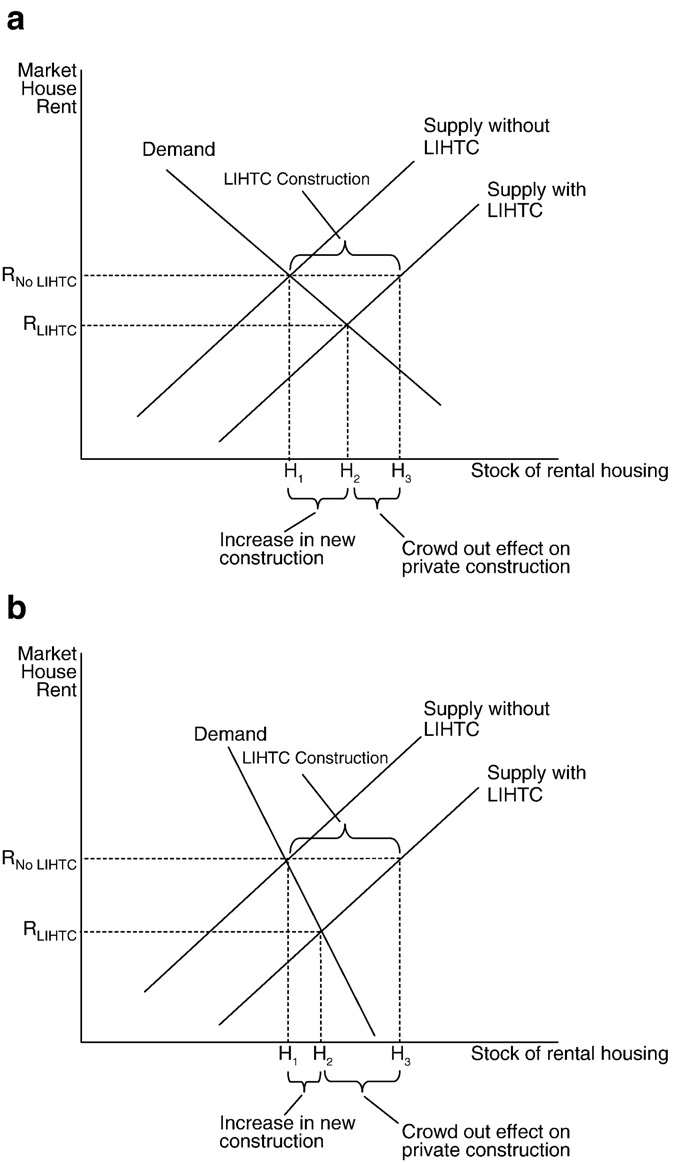
\includegraphics[width=11cm]{fig2.png}
	\caption{a: 有弹性需求的出租房被挤出,b: 因需求缺乏弹性而被挤出出租房}\label{fig2}
\end{figure}

现在考虑\figref{fig2}a,其描绘了在给定时间点的租赁房屋存量的市场。从LIHTC项目的一些细节中抽象出来,该项目资助的建设项目达到了外来的州级拨款。这意味着出租房屋总供给的向外转移,导致均衡租金下降,房屋存量增加\,\footnote{\figref{fig2}a 和 b 表明,LIHTC计划导致整个供应功能移出。这一简化抓住了LIHTC计划的主要影响。更准确的描述是,LIHTC计划将供应曲线最下部的斜率展平,直至分配给给定位置的LIHTC单位的最大数量。超过这一水平的建设,供应函数变陡,因为额外的投资是没有补贴的。这样的规范意味着开发商选择先投资LIHTC开发项目,然后再进行无补贴建设。此外,就LIHTC发展从非补贴部门吸引低成本要素投入而言,非补贴部门的投入成本将高于没有LIHTC计划的情况。这将导致供应功能的未补贴部分向内旋转。关于这个问题的进一步讨论,参见 \cite{Olsen2007618}。}。

在\figref{fig2}a中,请注意,LIHTC的开发压低了市场租金,导致出租房屋的总存量增加少于LIHTC建筑的水平($\rm{H}_2-\rm{H}_1 < \rm{H}_3-\rm{H}_1$)。不同的是,$\rm{H}_3-\rm{H}_2$代表了被LIHTC项目“挤出”的无补贴私人建筑。此外,\figref{fig2}b表示了随着需求函数变得更加无弹性,挤出变得更加明显。事实上,只有当住房需求完全弹性或者新建住房供应完全非弹性时,$\rm{H}_3-\rm{H}_2$等于零,挤出效应才会发生。

为了正确理解这一点,\cite{Hanushek1980449} 使用了20世纪70年代住房补贴实验的数据来估计出租房需求的弹性。匹兹堡和凤凰城的估计值分别$-0.36$和$-0.41$。对于自住单元,\cite{Rosen19791} 估计自住者随机样本的价格弹性为$-0.99$,而 \cite{Rosen19791} 估计FHA购房者的价格弹性为$-0.5$,这一群体的收入更接近于典型的租房者。这些估计证实,住房需求远非完全弹性。

在供给方面,\cite{Mayer200085} 估计,所有类型新建住房的供给弹性大约为6。这与 \cite{DiPasquale1992337} 估计的新建多户出租住房的供给弹性为6.8十分接近。对新建住房供应弹性的其他估计较小,但通常远高于1(例如 \citep{DiPasquale1992337,Rosen19791})。虽然以前估计的供给弹性范围比需求方面的变化更大,但考虑到住房存量的扩张,供给似乎远非完全无弹性\,\footnote{从另一个角度来看,如果可开发土地充足,而实际建筑成本不变,那么新的住房供应应该是完全有弹性的(例如 \citep{Rosenthal1994182})。这与住房存量的收缩形成对比,因为住房的耐久性意味着供应是非弹性的(例如 \citep{Glaeser2005345})。}。

总而言之,只有当住房需求完全弹性化或住房供给完全非弹性化时,挤出效应才会发生。然而,文献中的估计强烈表明这两种情况都不成立。除了记录在案的以中等收入家庭为目标的LIHTC计划的趋势,这表明在质量的基础上,LIHTC发展的倡导者和反对者都应该预计到该计划的排挤。问题是,多少钱?

\section{数据和实证模型}

\subsection{数据}

我们使用十年一次的人口普查数据作为我们控制变量的根数据源。这些数据是从1990年和2000年的地理信息系统公司邻域变化数据库文件中获得的\,\footnote{请参见 \url{http://www.geolytics.com}。}。地理信息系统公司将这些年的数据重新编码到2000年人口普查区域边界。这些数据与截至2000年投入使用的LIHTC项目的信息相结合。LIHTC的数据是通过互联网从住房和城市发展部获得的\,\footnote{请参见 \url{http://www.lihtc.huduser.org}。}。LIHTC数据库的信息包括投入使用的年份和2000年人口普查范围。我们的数据包括17,774个LIHTC项目,包含877,972个单元。

根据这些数据,我们进行了前面提到的三组分析。在第一种情况下,所有的数据都被汇总到MSA级别,MSA是一个足够大的地理单元,以至于在介绍中描述的方式跨社区的大多数交互都可能被考虑在内。对于分析的这一部分,我们从样本中删除非MSA区域。在第二种方法中,我们将数据聚集到县一级。虽然在地理上没有管理服务协定大,但有更多的县,这增加了数据的变化,有助于识别LIHTC排挤效应。此外,尽管我们在MSA层面的分析中包括了州固定效应,但对于县一级的回归,我们可以使用MSA和州特定的非MSA固定效应。

对于我们的最终方法,我们使用地理信息系统(GIS)软件将数据重组为半径10英里的统一圆形单位,每个圆围绕2000年人口普查的单个地理质心$i$ ($i = 1, \dots,n$)\,\footnote{MapInfo和MapBasic用于处理数据的地理特征。当在人口普查道质心周围画圆时,比例和度量被用来计算各种计数变量。}。为所有因变量和自变量以及构造我们的工具时使用的总体变量生成了基于圆的度量。 这样可确保用于测量回归方程两侧的变量的地理位置相同。 值得注意的是,典型的县所覆盖的区域少于半径10英里的圆圈。 出于这个原因,部分原因是,我们认为10英里范围内的措施至少在与县进行跨社区互动方面做得很好。 此外,由于圆圈是围绕基础普查区的地理质心绘制的,因此许多不同的圆圈都位于给定县内。 这使我们能够控制县级固定效应,并进一步加强识别。 为了考虑圆的重叠性质并隐含重复因变量中的某些信息,我们在县一级对圆回归中的标准误差进行了聚类。 \figref{tab3}提供了州级,县级和10英里圈数据的摘要统计数据。


%\nocite{*}
\bibliography{ref}

\appendix
\appendixpage
\addappheadtotoc
\section{How I became inspired}


\end{document}
